%%%%% Begin LaTeX Beamer Preamble %%%%%

  \documentclass[9pt]{beamer}

  \usetheme{Goettingen} % Or use Luebeck (different bullet points from Malmoe)
  % other themes: AnnArbor, Antibes, Bergen, Berkeley, Berlin, Boadilla, boxes, CambridgeUS, Copenhagen, Darmstadt, default, Dresden, Frankfurt, Goettingen, Hannover, Ilmenau, JuanLesPins, Luebeck, Madrid, Malmoe, Marburg, Montpellier, PaloAlto, Pittsburg, Rochester, Singapore, Szeged, default, classic

  \usefonttheme{professionalfonts}
  %font themes: default, professionalfonts, serif (Times New Roman), structurebold, structureitalicserif, structuresmallcapsserif

  \usecolortheme{seahorse} % Other tolerable color schemes rose, whale, orchid, dolphin, lily
  % color themes: albatross, beaver, beetle, crane, default, dolphin, dove (black and white), fly (gray and white), lily, orchid, rose, seagull (gray), seahorse (light blue), sidebartab, whale, wolverine

  %\setbeamercovered{transparent} % Given overlays, pauses and similar, this command allows you to specify in a quite general way how a covered item should be rendered

  \setbeamertemplate{navigation symbols}{\textcolor{black}{{\footnotesize \insertframenumber/\inserttotalframenumber}}} % Removes navigation tools and adds slide number/total slide count at bottom right
  %\setbeamertemplate{navigation symbols}{} % Just removes navigation tools

  %\setbeamertemplate{bibliography item}[article] % Changes the bibliography item icon, options: article, book, ...
  \setbeamertemplate{bibliography item}{} % No bibliography item icon

  \setbeamertemplate{caption}[numbered] % Option to have the figures numbered

  \useoutertheme[subsection=false]{smoothbars} % Suppress subsections

  % New command, math operator declarations
  \DeclareMathOperator*{\argmax}{argmax}
  \DeclareMathOperator*{\argmin}{argmin}

  % Packages
  \usepackage{amsmath, amsthm, amssymb}
  \usepackage[english]{babel}
  \usepackage[latin1]{inputenc}
  \usepackage[T1]{fontenc}
  \usepackage{times}
  \usepackage{color}
  \usepackage{verbatim}
  \usepackage{graphicx}
  \usepackage{bm}
  \usepackage[all]{xy}
  \usepackage[latin1]{inputenc}
  \usepackage{hyperref}
  
%\usepackage{enumitem}
%\setenumerate[1]{label=\arabic*.}
%\newcounter{ResumeEnumerate}
  % Presentation meta-information
  \title[Bayesian Approach in HIV Dynamical Models]{Bayesian Approach in HIV Dynamical Models}
  \author[Wei Cui]{Wei Cui  { \texttt{}}}


  \institute{~\\Department of Statistics \\University of California, Riverside}
  
  \date{\small{April 17th, 2015}}
  \subject{Slide Presentation} % Enters option text as the subject text in the pdf document info

%%%%% End LaTeX Beamer Preamble %%%%%

\begin{document} %%%%%%%



\begin{frame} %%%
  \titlepage
\end{frame} %%%



% Do a brief overview of the talk here before getting into it.
\begin{frame}{Outline} %%%
%\begin{frame}[allowframebreaks]{Outline}
  \tableofcontents
\end{frame} %%%

\section[Background]{Background}
\subsection[HIV]{HIV}
\begin{frame}{Life Cycle of HIV}
  \begin{figure}
    \centering
    \def\svgwidth{\columnwidth}
    \input{HIVReplicationCycle.pdf_tex}
  \end{figure}
"\href{http://en.wikipedia.org/wiki/HIV\#/media/File:HIV-replication-cycle.svg}{The HIV replication cycle}" by \href{http://commons.wikimedia.org/wiki/User:Splette}{Thomas Splettstoesser} is licensed under \href{http://creativecommons.org/licenses/by-sa/3.0/}{CC BY-SA 3.0}
\end{frame}

\begin{frame}{HIV RNA Copies and CD$4^{+}$ Count}
  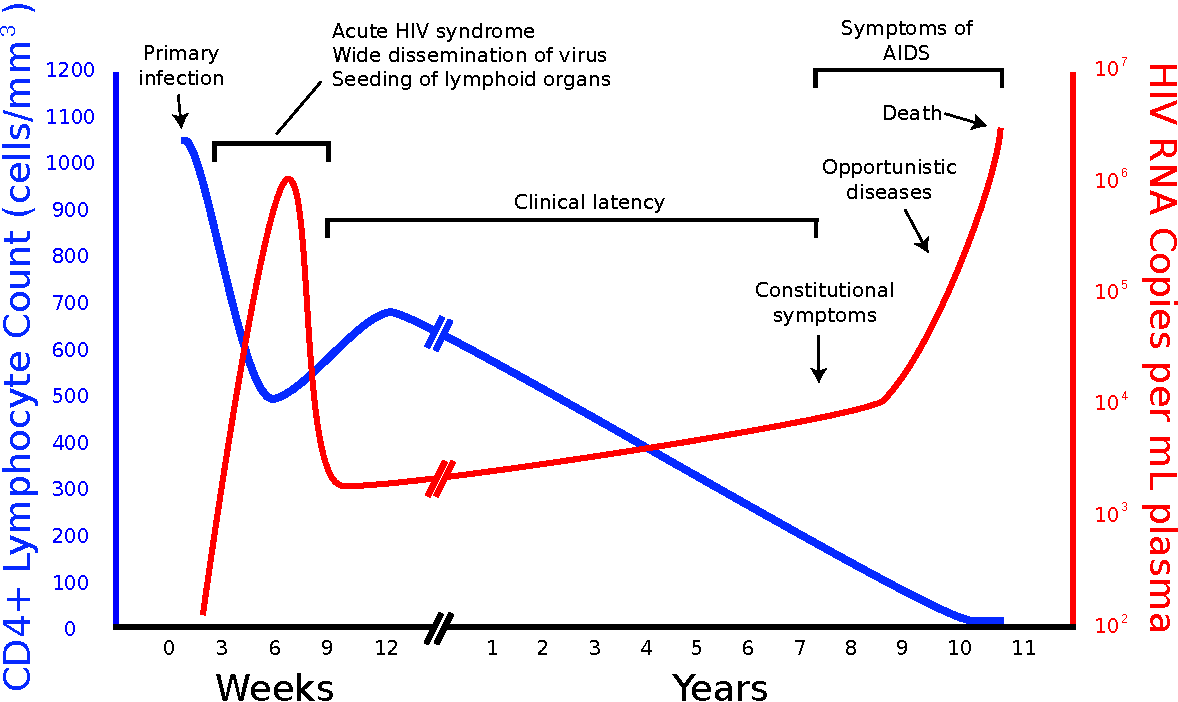
\includegraphics[scale=0.5]{Hiv-timecourse_copy}
\end{frame}

\subsection[Basic Model]{Basic Model}
\begin{frame}{The Basic HIV Dynamic Model}
The basic HIV dynamic model is a model that describes the population dynamics of HIV and its target cells in plasma.
\begin{equation}
\begin{array}{rcl}
\frac{dT}{dt} & = & \lambda{}-\rho{}T-kTV \\ \\
\frac{dT^{*}}{dt} & = & kTV-\delta{}T^{*} \\ \\
\frac{dV}{dt} & = & N\delta{}T^{*}-cV
\end{array}
\end{equation}
where $T$, $T^{*}$ and $V$ are target uninfected CD4+ T cells, infected CD4+ T cells and virus, respectively.  $\rho$, $\delta$, $c$ are death rate of target uninfected CD4+ T cells, infected CD4+ T cells and virus, respectively. $\lambda$ represents the produce rate of new CD4+ T cells from body, k is the infected rate and N is the number of new virions produced from each (death) infected T cell.
\end{frame}

\begin{frame}{The Solution of the Basic Model}
\begin{equation}
R_{0}=\frac{\lambda{}kN}{\rho{}c}
\end{equation}
When $R_{0}>1$, the system will reach some equilibrium status as following
\begin{equation}
\begin{array}{rcl}
T_{0} & = & \frac{c}{kN} \\ \\
V_{0} & = & \frac{\lambda{}N}{c}-\frac{\rho}{k} \\ \\
T_{0}^{*} & = & \frac{c}{\delta{}N}
\end{array}
\end{equation}
This is the initial values of all the HIV dynamic models with antiviral. 
\end{frame}

\begin{frame}{Problems of the Basic Model}

\end{frame}

\subsection[Drugs]{Drugs}
\begin{frame}{Review the Life Cycle of HIV}
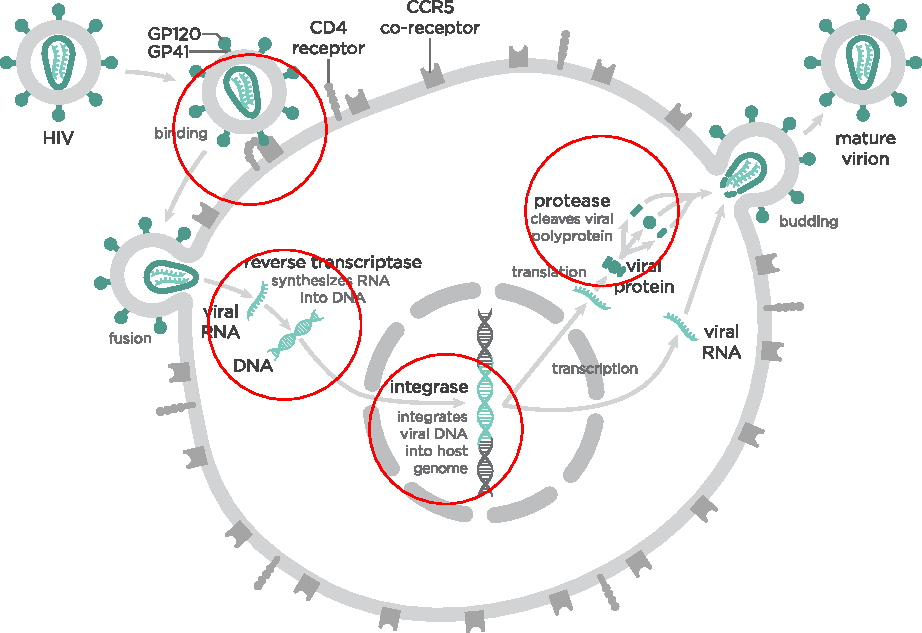
\includegraphics[scale=0.65]{HIV-replication-cycle-modify} \\
Modified by Wei Cui from "\href{http://en.wikipedia.org/wiki/HIV\#/media/File:HIV-replication-cycle.svg}{The HIV replication cycle}" by \href{http://commons.wikimedia.org/wiki/User:Splette}{Thomas Splettstoesser} licensed under \href{http://creativecommons.org/licenses/by-sa/3.0/}{CC BY-SA 3.0}
\end{frame}

\begin{frame}{Approved Drugs by FDA}
There are four kinds of drugs approved by FDA \\
1. Entry inhibitor \\
2. Reverse transcriptase inhibitor \\
3. Integrase inhibitor \\
4. Protease inhibitor 
\end{frame}

\section[Models]{Antiviral Models}
\subsection[Models]{Models}
\begin{frame}{General Model}
\begin{equation}
\begin{array}{rcl}
\frac{dT}{dt} & = & {\color{red}\lambda{}(t)}-\rho{}T-{\color{red}(1-\gamma{}_{RTI}(t))}kTV \\ \\
\frac{dT^{*}}{dt} & = & {\color{red}(1-\gamma{}_{RTI}(t))}kTV-\delta{}T^{*} \\ \\
\frac{dV}{dt} & = & {\color{red}(1-\gamma{}_{PI}(t))}N\delta{}T^{*}-cV \\ \\
\frac{dU}{dt} & = & {\color{red}\gamma{}_{PI}(t)N\delta{}T^{*}-cU} \label{generalmodel}
\end{array}
\end{equation}
\\
$\eta{}_{RTI}(t)$ indicates the fraction of new infections inhibited. \\
$\eta{}_{PI}(t)$ denotes the fraction of virus produced being non-infectious. 
\end{frame}

\begin{frame}{Putter's Model}
\begin{equation}
\begin{array}{rcl}
\frac{dT}{dt} & = & \lambda{}-\rho{}T-{\color{red}(1-\gamma{})}kTV \\ \\
\frac{dT^{*}}{dt} & = & {\color{red}(1-\gamma{})}kTV-\delta{}T^{*} \\ \\
\frac{dV}{dt} & = & {\color{red}(1-\gamma{})}N\delta{}T^{*}-cV \\ \\
\frac{dU}{dt} & = & {\color{red}\gamma{}}N\delta{}T^{*}-cU \label{Puttermodel}
\end{array}
\end{equation}
\\
Putter, H., et al., 
\emph{A Bayesian approach to parameter estimation in HIV}. 
dynamical models. Stat Med, 2002. 21(15): p. 2199-214.
\end{frame}

\begin{frame}{Huang's Model}
\begin{equation}
\begin{array}{rcl}
\frac{dT}{dt} & = & \lambda{}-\rho{}T-(1-\gamma{}(t))kTV \\ \\
\frac{dT^{*}}{dt} & = & (1-\gamma{}(t))kTV-\delta{}T^{*} \\ \\
\frac{dV}{dt} & = & N\delta{}T^{*}-cV  \label{Huangmodel} \\ \\
\gamma{}(t) & = & {\color{red}\frac{C_{min}A(t)}{\phi{}IC_{50}(t)+C_{min}A(t)}}
\end{array}
\end{equation}

$IC_{50}$ represents the drug concentration necessary to inhibit viral replication by $50\%$. \\
$C_{min}$ is the minimum concentration of drug in plasma. \\
$A(t)$ is indicator of doses to patients, $\phi$ indicates a conversion factor. \\
Huang, Y. and H. Wu, 
\emph{A bayesian approach for estimating antiviral efficacy in HIV dynamic models}. 
J Applied Statistics, 2006. 33: p. 155-174.
\end{frame}

\section[Solution of Huang's Model]{Solution of Huang's Model}
\subsection{Nonlinear Mixed Effects Model}
\begin{frame}{Parameters}
\begin{equation}
\begin{array}{rcl}
\mu & = & (log\phi{},logc,log\delta{},log\lambda{},log\rho{},logN,logk)^{T}, \\
\Theta & = & \{\theta_{i},i=1,\ldots,n\}, \\
\theta_{i} & = & (log\phi{}_{i},logc_{i},log\delta{}_{i},log\lambda{}_{i},log\rho{}_{i},logN_{i},logk_{i})^{T}, \\
\Theta_{\{i\}} & = & \{\theta_{l},l\neq{}i\}, \\
Y & = & \{y_{ij},i=1,\ldots,n;j=1,\ldots,m_{i}\}
\end{array}
\end{equation}
Let $f_{ij}(\theta_{i},t_{j})$ be logarithm of the (numeric) solution of $V$ from \eqref{specificmodel} for the $i$th subject at time $t_j$. The repeated measurements of it, $y_{ij}(t)$ can be written as
\begin{equation}
y_{ij}(t_{j})=f_{ij}(\theta_{i},t_{j})+e_{i}(t_{j}), i=1,\ldots,n;j=1,\ldots,m_{i}
\end{equation}
where $e_{i}(t)$ is a measurement error with mean zero. 
\end{frame}

\begin{frame}{Three Stage Hierarchical Model}
Stage 1.
Within-subject variation in common logarithmic viral load measurements which is the individual model:
\begin{equation}
y_{i}=f_{i}(\theta{}_{i})+e_{i}, [e_{i}|\sigma{}^{2},\theta{}_{i}]\sim{}N(0,\sigma{}^{2}I_{m_i})
\end{equation}
Stage 2.
Between-subject variation which is the population model:
\begin{equation}
\theta_{i}=\mu+b_{i}, [b_{i}|\Sigma]\sim{}N(0,\Sigma)
\end{equation}
Stage 3.
Hyperprior distribution:
\begin{equation}
\sigma^{-2}\sim{}Ga(a,b), \mu\sim{}N(\eta,\Lambda), \Sigma{}^{-1}\sim{}Wi(\Omega,v)
\end{equation}
\end{frame}


\begin{frame}{Conditional Distribution}
\begin{equation}
\begin{array}
[\sigma{}^{-2}|\mu{},\Sigma{}^{-1},\Theta{},Y] \sim{} \\
Ga\left(a+\frac{\sum_{i=1}^{n}m_{i}}{2},\left\{\frac{1}{b}+\frac{1}{2}\sum_{i=1}^{n}\sum_{j=1}^{m_{i}}[y_{ij}-f_{ij}(\theta_{i},t_{j})]^{2}\right\}^{-1}\right) \\
[\mu{}|\sigma{}^{-2},\Sigma{}^{-1},\Theta{},Y] \sim{}
N\left((n\Sigma^{-1}+\Lambda^{-1})^{-1}(\Sigma^{-1}\sum_{i=1}^{n}\theta_{i}+\Lambda^{-1}\eta),(n\Sigma^{-1}+\Lambda^{-1})^{-1}\right)

[\Sigma{}^{-1}|\sigma{}^{-2},\mu{},\Theta{},Y] \sim{} \\
Wi\left(\left[\Omega^{-1}+\sum_{i=1}^{n}(\theta-\mu)(\theta-\mu)^{T}\right]^{-1},n+v\right) \\ \\
[\theta_{i}|\sigma{}^{-2},\mu{},\Sigma{}^{-1},\Theta{}_{\{i\}},Y] \sim{} \\ 
exp\left\{-\frac{\sigma^{-2}}{2}\sum_{j=1}^{m_{i}}[y_{ij}-f_{ij}(\theta_{i},t_{j})]^{2}-\frac{1}{2}(\theta-\mu)^{T}\Sigma^{-1}(\theta-\mu)\right\}

\end{array}
\end{equation}
\end{frame}


\subsection{MCMC}
\begin{frame}{}
Step 1.
Initialize the iteration counter to $j=1$ and start with initial values $\Gamma{}^{(0)}=(\sigma{}^{-2(0)},\mu{}^{(0)},\Sigma{}^{-1(0)},\Theta{}^{(0)})^{T}$.
Step 2.
Obtain a new value  $\Gamma{}^{(j)}=(\sigma{}^{-2(j)},\mu{}^{(j)},\Sigma{}^{-1(j)},\Theta{}^{(j)})^{T}$ from $\Gamma{}^{(j-1)}$ through successive generation of values:
Step 2.1 Gibbs sampling.
\begin{equation}
\begin{array}{rcl}
\sigma{}^{-2(j)} & \sim{} & \pi{}(\sigma^{-2}|\mu{}^{(j-1)},\Sigma{}^{-1(j-1)},\Theta{}^{(j-1)},Y) \\
\mu{}^{(j)} & \sim{} & \pi{}(\mu{}|\sigma{}^{-2(j-1)},\Sigma{}^{-1(j-1)},\Theta{}^{(j-1)},Y) \\
\Sigma{}^{-1(j)} & \sim{} & \pi{}(\Sigma{}^{-1}|\sigma{}^{-2(j-1)},\mu{}^{(j-1)},\Theta{}^{(j-1)},Y)
\end{array}
\end{equation}
Step 2.2 Metropolis-Hastings step.
For $\theta{}_{i}^{(j)}$, generate a new value $\varphi$ from the proposal (symmetric) density $q(\varphi{}|\theta{}_{i}^{(j-1)})$, calculate
\begin{equation}
\alpha{}(\varphi{}|\theta{}_{i}^{(j-1)})=\frac{\pi{}(\varphi{}|\sigma{}^{-2(j)},\mu{}^{(j)},\Sigma{}^{-1(j)},\Theta{}_{\{i\}}^{(j-1)},Y)}{\pi{}(\theta{}_{i}^{(j-1)}|\sigma{}^{-2(j)},\mu{}^{(j)},\Sigma{}^{-1(j)},\Theta{}_{\{i\}}^{(j-1)},Y)}
\end{equation}
If $\alpha{}(\varphi{}|\theta{}_{i}^{(j-1)})\ge{}1$ then accept it,$\theta{}_{i}^{(j)}=\varphi{}$. If $\alpha{}(\varphi{}|\theta{}_{i}^{(j-1)})<1$ then also accept it with a given probability.
Step 3.
Change the counter from $j$ to $j+1$ and return to Step 2 until convergence is reached.
\end{frame}

\end{document} %%%%%%%
